\documentclass{article}
\usepackage[a4paper, margin=1in]{geometry}
\usepackage[T1]{fontenc}
\usepackage[utf8]{inputenc}
\usepackage{amsmath, amssymb, graphicx, hyperref}
\graphicspath{{../figures/}}
\usepackage[framed,numbered]{matlab-prettifier}
\usepackage{xcolor}
\usepackage{bookmark}
\usepackage{listings}

\geometry{a4paper, margin=1in}

% MATLAB code style
\lstset{
  style      = Matlab-editor,
  basicstyle = \mlttfamily,
  breaklines = true
}

\title{\textbf{Practical - 12}}
\author{}
\date{October 29, 2026}

\pagenumbering{gobble}

\begin{document}
\maketitle

\noindent
\textbf{\large{Aim:}} To analyze epidemic models of influenza, including basic epidemic models, lifelong contagiousness, and disease transmission with carriers.

\vspace{1em}
\noindent
\textbf{\large{Theory:}}

\vspace{0.5em}
\noindent
\underline{INTRODUCTION}

\noindent
The SIR model divides a population into three groups:
\begin{itemize}
    \item \textbf{S - Susceptible:} People who can catch influenza.
    \item \textbf{I - Infected:} People who currently have influenza and can spread it.
    \item \textbf{R - Recovered:} People who are recovered and are assumed not to be infectious during the modelled period.
\end{itemize}

\vspace{0.5em}
\noindent
\underline{Assumptions and Precautions}

\noindent
The parameter values are chosen for demonstration and should not be treated as real influenza estimates.

\noindent
The model does not include births, migration, or deaths unrelated to the disease.

\noindent
The basic SIR model assumes recovered individuals do not return to the susceptible group during the simulated period.

\vspace{1.5em}
\noindent
\textbf{Mathematical model}

    \[\frac{dS}{dt} = \frac{-\beta S I}{N}\]
    \[\frac{dI}{dt} = \frac{\beta S I}{N} - \gamma I\]
    \[\frac{dR}{dt} = \gamma I\]

\noindent
Here, $N = S + I + R$ is the total population, $t$ is time in days, $\beta$ is the transmission parameter, and $\gamma$ is the recovery parameter. The term $\frac{\beta S I}{N}$ represents new infections per unit time, while $\gamma I$ represents recoveries per unit time. This basic model assumes a closed population.

\newpage
\noindent
\textbf{\large{MATLAB Code:}}
\begin{lstlisting}
clc; clear all; close all;

% Model Parameters
N = 1000;
beta = 0.3;
gamma = 0.1;

% Initial Populations
S0 = 990;
I0 = 10;
R0 = 0;

% Time interval in days
tspan = [0 100];

% Initial Conditions
initial = [S0; I0; R0];

% SIR Differential Equations
f = @(t,z)[-beta*z(1)*z(2)/N;
    beta*z(1)*z(2)/N - gamma*z(2);
    gamma*z(2)];

% Solve the differential equations numerically
[t,Z] = ode45(f, tspan, initial);

% Extract the solutions
S = Z(:,1);
I = Z(:,2);
R = Z(:,3);

% Plot the results
plot(t,S,'LineWidth',1.5);
hold on
plot(t,I,'LineWidth',1.5);
plot(t,R,'LineWidth',1.5)
grid on
xlabel('Time(days)');
ylabel('Number of Individuals');
title('Basic SIR Model of Influenza');
legend('Susceptible','Infected','Recovered','Location','best');
hold off
\end{lstlisting}

\vspace{1em}
\noindent
\textbf{\large{Output:}}
\begin{figure}
\centering
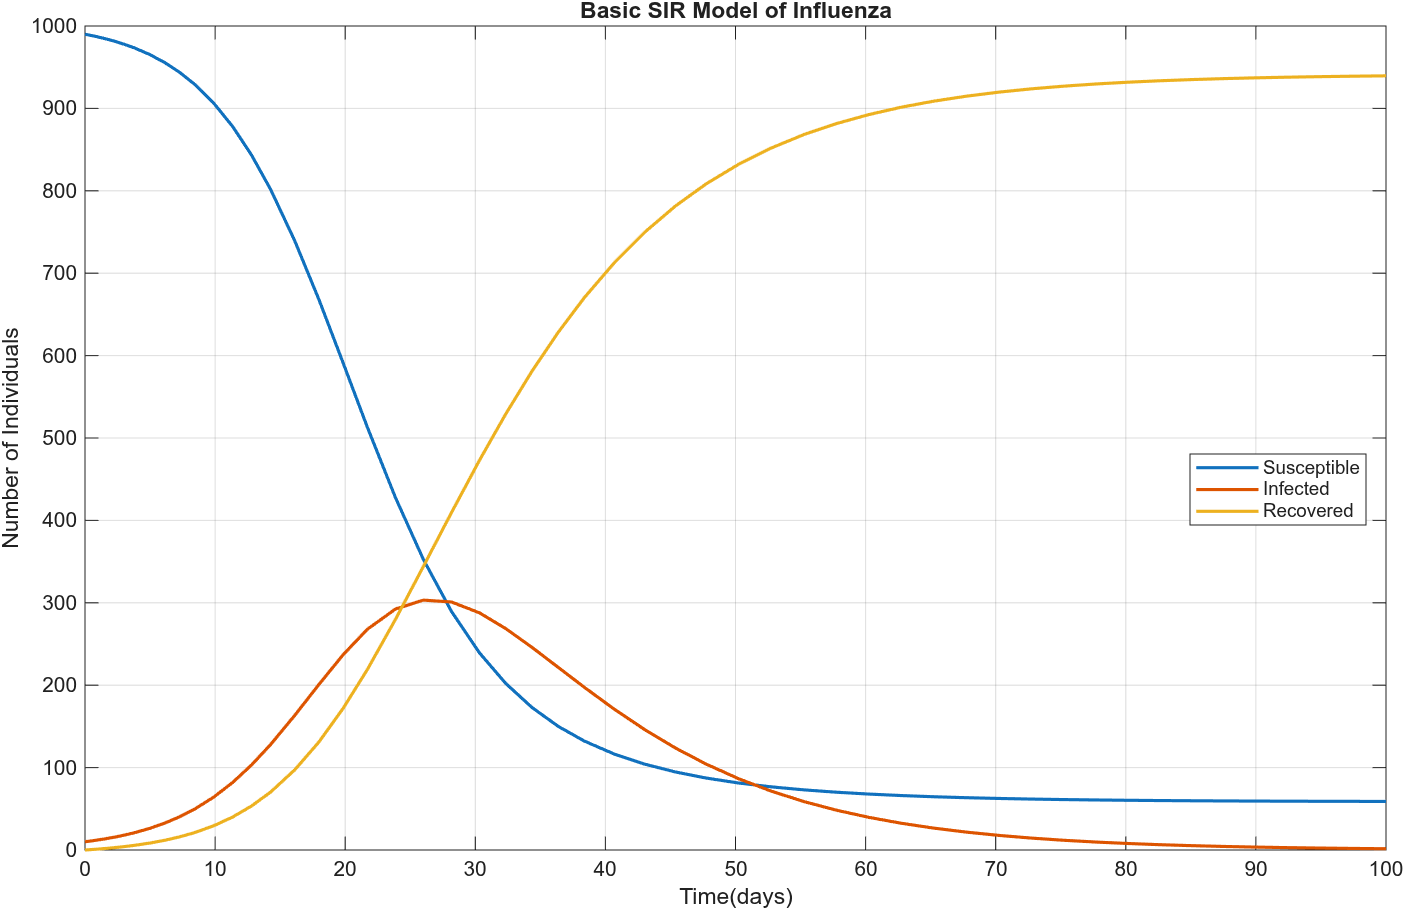
\includegraphics[width=0.7\textwidth]{Figure12.png}
\end{figure}

\newpage
\noindent
\textbf{\large{Graph and Interpretation:}}
\begin{itemize}
    \item The suspectible population generally decreases as people become infected.
    \item The infected population may first increase, reach a peak, and then decrease as transmission slows and infected people recover.
    \item The recovered population increases as infected people recover.
    \item The total $S + I + R$ should remain approximately 1000, allowing for small numerical rounding errors.
\end{itemize}

\end{document}
